\section{Hashing}
Um eine \textit{Adresse} für ein zu speicherndes Elemente zu berechnen, werden \textbf{Hashverfahren} genutzt.\\
Der Wert des zu speichernden Elementes dient dabei als Grundlage zur Berechnung der Adresse.\\
Der Speicher, in dem die Elemente abgelegt werden soll, bezeichnet man dabei als \textit{buckets}: $B_0,\dots , B_{m - 1}$ (vgl.~\cite[115]{GD18d}).\\

\noindent
Es wird unterschieden zwischen \textbf{geschlossenem} und \textbf{offenem} Hashing (vgl.~\cite[116]{GD18d}): Bei offenem Hashing werden Überläufer verkettet, bei geschlossenem Hashing kann es zu Kollisionen mit bereits belegten Adressen können - über \textbf{rehashing}\footnote{
auch: \textit{offene Adressierung} (vgl.~\cite[119]{GD18d})
}) können Adressen neu berechnet werden, woraus sich \textbf{Sondierungsfolgen} ergeben.\\

\noindent
Während bei offenem Hashing $m$ Buckets ihre Überläufer jeweils einfach in einer verketteten Liste speichern, ist die Anzahl der jeweils speicherbaren Elemente durch $b$ begrenzt.
Bei \textit{geschlossenem Hashing} wird oft der Spezialfall $b = 1$ betrachtet; trotzdem kann auch bei geschlossenem Hashing durchaus $b > 1$ sein (s. Abbildung~\ref{fig:openaddressing}).\\

\begin{figure}
\begin{center}
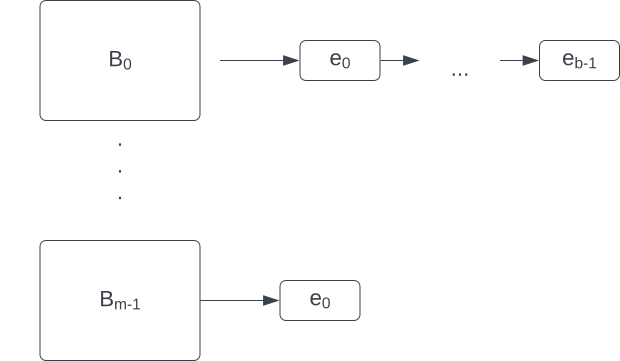
\includegraphics[scale=0.4]{chapters/Datenstrukturen und Algorithmen/img/openaddressing}
\caption{Die Abbildung stell schematisch geschlossenes Hashing dar. Hierbei ist die Anzahl der speicherbaren Elemente mit $b$ pro Bucket begrenzt, sodass sich die zur Verfügung stehenden Speicherplätze aus $m * b$ berechnen. Bei offenem Hashing werden Überläufer hingegen einfach in verketteten Listen gespeichert. (Quelle: eigene)}
\label{fig:openaddressing}
\end{center}
\end{figure}

\subsection{Hashfunktionen}

Für die Berechnung einer Adresse wird oft der \textit{modulo}-Operator verwendet

\begin{equation}
    b\ mod\ m
\end{equation}

\noindent
für den wie folgt gilt\footnote{
s. a. ``Modulo``: \url{https://de.wikipedia.org/wiki/Division_mit_Rest#Modulo} - abgerufen 09.03.2024
}:

\begin{equation}
    b\ mod\ m = b - \lfloor \frac{m}{b} \rfloor * m
\end{equation}

\subsection*{Beispiele}

\begin{itemize}
    \item $-1\ mod\ 7 = -1 - \lfloor \frac{-1}{7} \rfloor * 7 =  -1 - (-1 * 7) = 6$
    \item $19\ mod\ 7 = 19 - \lfloor \frac{19}{7} \rfloor * 7 =  19 - (2 * 7) = 5$
    \item $-8\ mod\ 6 = -8 - \frac{-8}{6} * 6 = -8 - (-2 * 6) = 4$
\end{itemize}

\subsection{Doppel-Hashing}
Bei \textfb{Doppel-Hashing} wird eine Sondierungsfunktion $s(k, i)$ benutzt, die eine zweite Hashfunktion $h_2(k)$ neben der eigentlichen Hashfunktion $h_1(k)$ verwendet.\\
Die Adresse für $k$ wird zunächst über $h_1(k)$ berechnet.
Kommt es zu einer Kollision, wird die \textit{Sondierungsfunktion} verwendet, beginnend mit $i=1$, bis keine weiteren Kollisionen auftreten\footnote{
s. a. ``Doppel-Hashing``: \url{https://de.wikipedia.org/wiki/Doppel-Hashing} - abgerufen 11.03.2024
}.


\subsection{Anmerkungen}
\textit{Ottmann und Widmayer} beschreiben unter \textit{Offene Hashverfahren} das geschlossene Hashing (vgl.~\cite[203 ff.]{OW17d}); \textit{Cormen et al.} bezeichnen behandeln dasselbe unter \textit{open adressing} in ~\cite[293 ff.]{CL22}.\\

\noindent
Bei\textit{Ottman und Widmayer} sind \textit{Hashverfahren mit Verkettung der Überläufer} (vgl.~\cite[198 ff.]{OW17d}) gleichzusetzen mit \textit{Sedgewick's und Wayne's} \textit{Hashing with separate  chaining} in ~\cite[464 ff.]{SW11} und wird bei \texit{Güting und Dieker} als \textit{offenes Hashing} bezeichnet (vgl.~\cite[116]{GD18d}).
